\chapter{Appendix}

\section{Source Code}
\subsection{Audio Watermarking Process}
\begin{lstlisting}
// Audio Watermarking Process
func (ms *MarkStream) Embedding(l []float64) {
	var i = SAMPLE_PER_FRAME - 1
	var j = 0

	for i < len(l) {
		select {
		case watermark := <-ms.userInputChan:
			var pos = 0
			submag := make([]float64, i+1-j)
			subphs := make([]float64, i+1-j)
			var stringbit = PrepareString("1" + watermark + "\n")
			for pos < len(stringbit) {
				var subl = l[j : i+1]
				subfourier := fft.FFTReal64(subl)
				var count = 0
				var bitrepeat = 0

				for k, x := range subfourier {
					submag[k], subphs[k] = cmplx.Polar(x)
					if submag[k] < MAG_THRES {
						continue
					}
					if pos < len(stringbit) && count < BIN_PER_FRAME {
						subphs[k] = QIMEncode(submag[k], subphs[k], int(stringbit[pos]))
						count++
						bitrepeat++
					}
					if bitrepeat == BIT_REPEAT {
						bitrepeat = 0
						pos++
					}
				}

				cmplxArray := make([]complex128, len(subl))
				for i, _ := range cmplxArray {
					cmplxArray[i] = cmplx.Rect(submag[i], subphs[i])
				}
				newWav := fft.IFFTRealOutput(cmplxArray)
				Wav16bit := Scale(newWav)
				ms.connManager.audioDataChan <- Wav16bit
				j = i + 1
				i += SAMPLE_PER_FRAME
				if len(l)-i > 0 && len(l)-i < SAMPLE_PER_FRAME {
					i = len(l) - 1
				}
				time.Sleep(400 * time.Millisecond)
			}
		default:
			var pos = 0
			var subl = l[j : i+1]
			subfourier := fft.FFTReal64(subl)
			submag := make([]float64, i+1-j)
			subphs := make([]float64, i+1-j)
			var stringbit = PrepareString("0")
			for pos < len(stringbit) {
				var count = 0
				var bitrepeat = 0

				for k, x := range subfourier {
					submag[k], subphs[k] = cmplx.Polar(x)
					if submag[k] < MAG_THRES {
						continue
					}
					if pos < len(stringbit) && count < BIN_PER_FRAME {
						subphs[k] = QIMEncode(submag[k], subphs[k], int(stringbit[pos]))
						count++
						bitrepeat++
					}
					if bitrepeat == BIT_REPEAT {
						bitrepeat = 0
						pos++
					}
				}

			}
			cmplxArray := make([]complex128, len(subl))
			for i, _ := range cmplxArray {
				cmplxArray[i] = cmplx.Rect(submag[i], subphs[i])
			}
			newWav := fft.IFFTRealOutput(cmplxArray)
			Wav16bit := Scale(newWav)
			ms.connManager.audioDataChan <- Wav16bit
			j = i + 1
			i += SAMPLE_PER_FRAME
			if len(l)-i > 0 && len(l)-i < SAMPLE_PER_FRAME {
				i = len(l) - 1
			}
			time.Sleep(400 * time.Millisecond)
		}
	}
}

\end{lstlisting}

\section{Images}
\begin{figure}[h]
	\centering
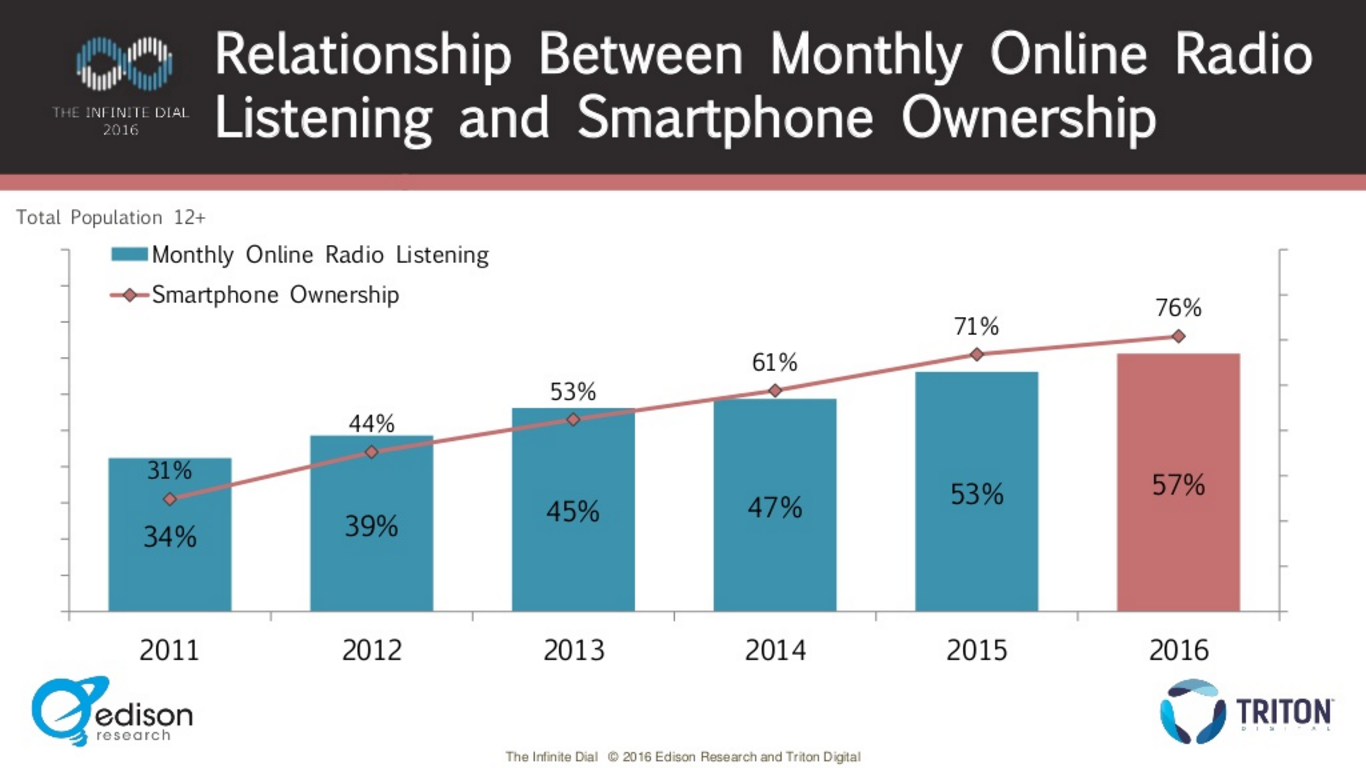
\includegraphics[width=\textwidth]{relation-monthly-mobile}
 	\caption{Relationship between monthly online radio listners and smartphone owners. Source \cite{edisonslide}}
 	\label{fig:MonthlyMobile}
\end{figure}
\begin{figure}[h]
	\centering
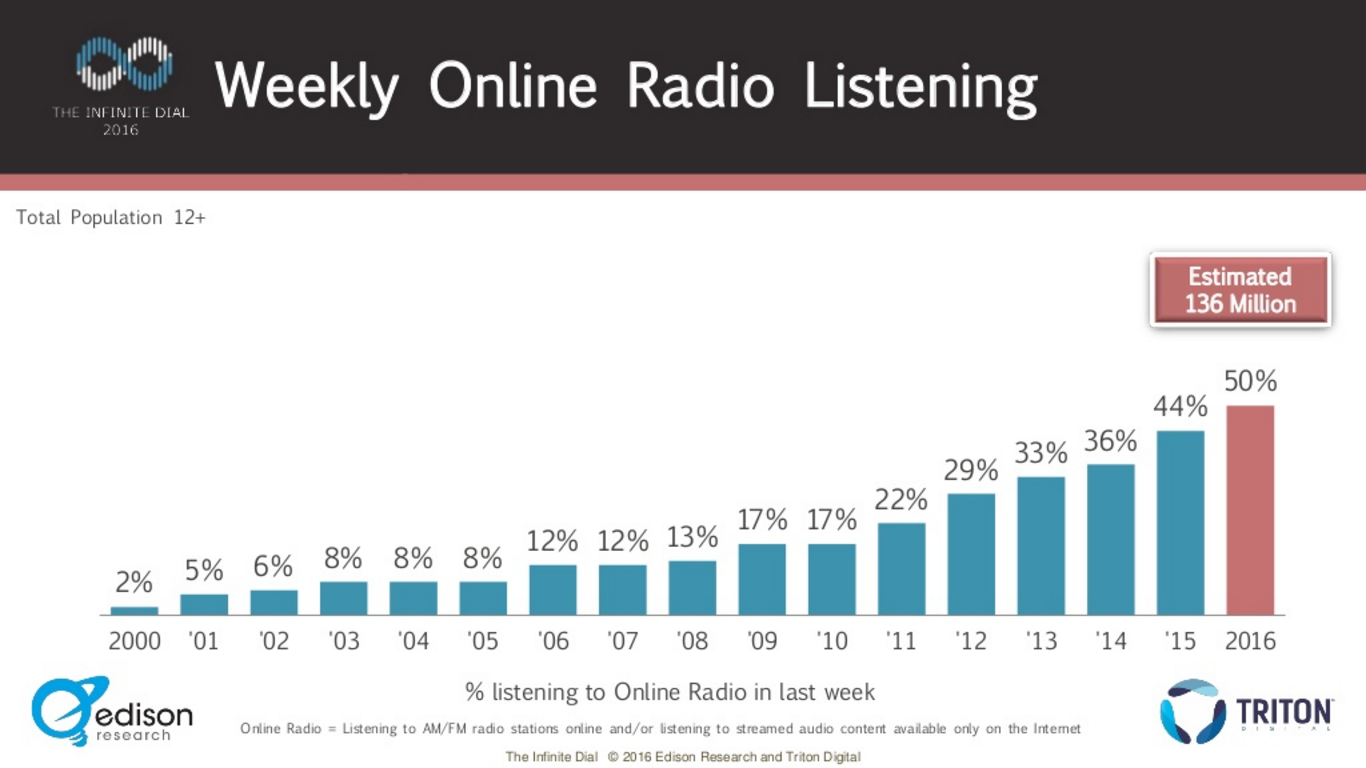
\includegraphics[width=\textwidth]{weekly-online-listening}
 	\caption{Weekly online radio listners. Source \cite{edisonslide}}
 	\label{fig:WeeklyListeners}
\end{figure}
\begin{figure}[h]
	\centering
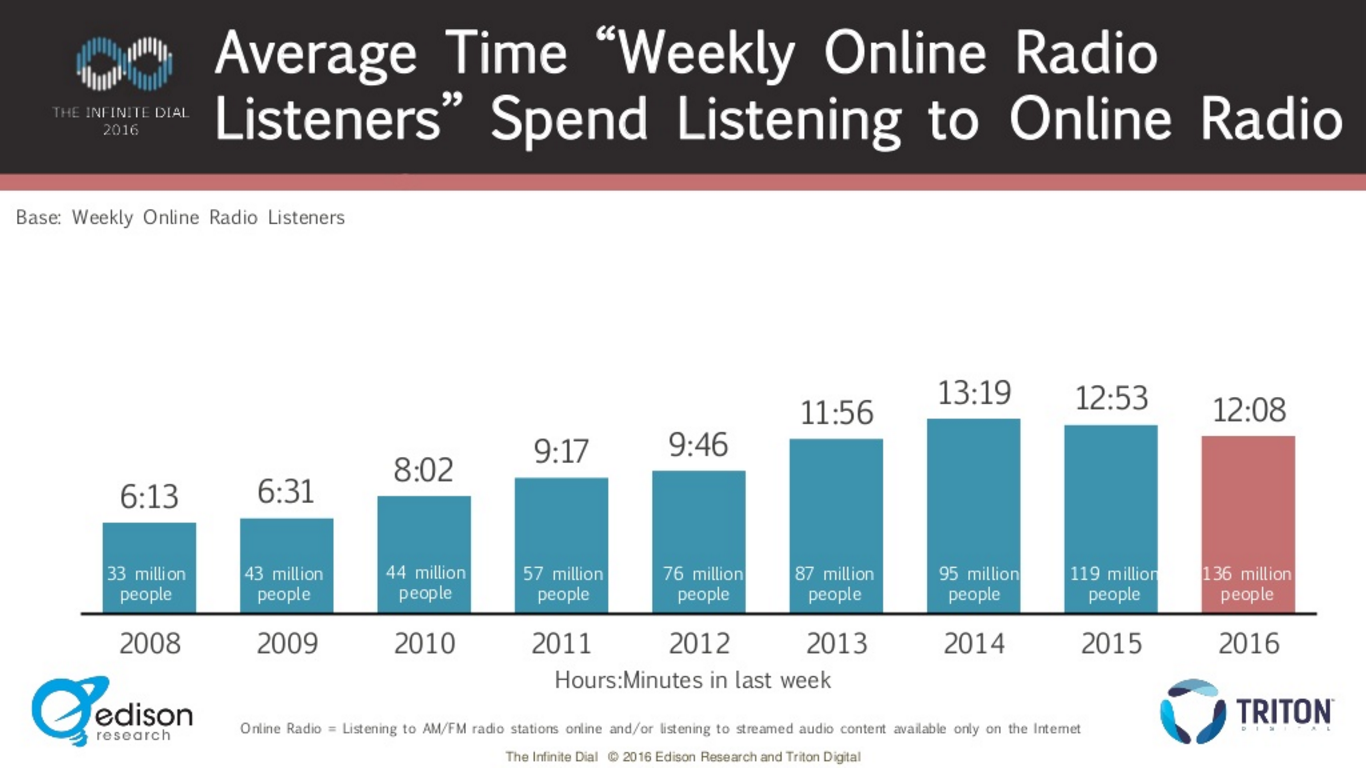
\includegraphics[width=\textwidth]{time-weekly}
 	\caption{Average time listening in a week. Source \cite{edisonslide}}
 	\label{fig:TimeWeekly}
\end{figure}
\begin{figure}[h]
	\centering
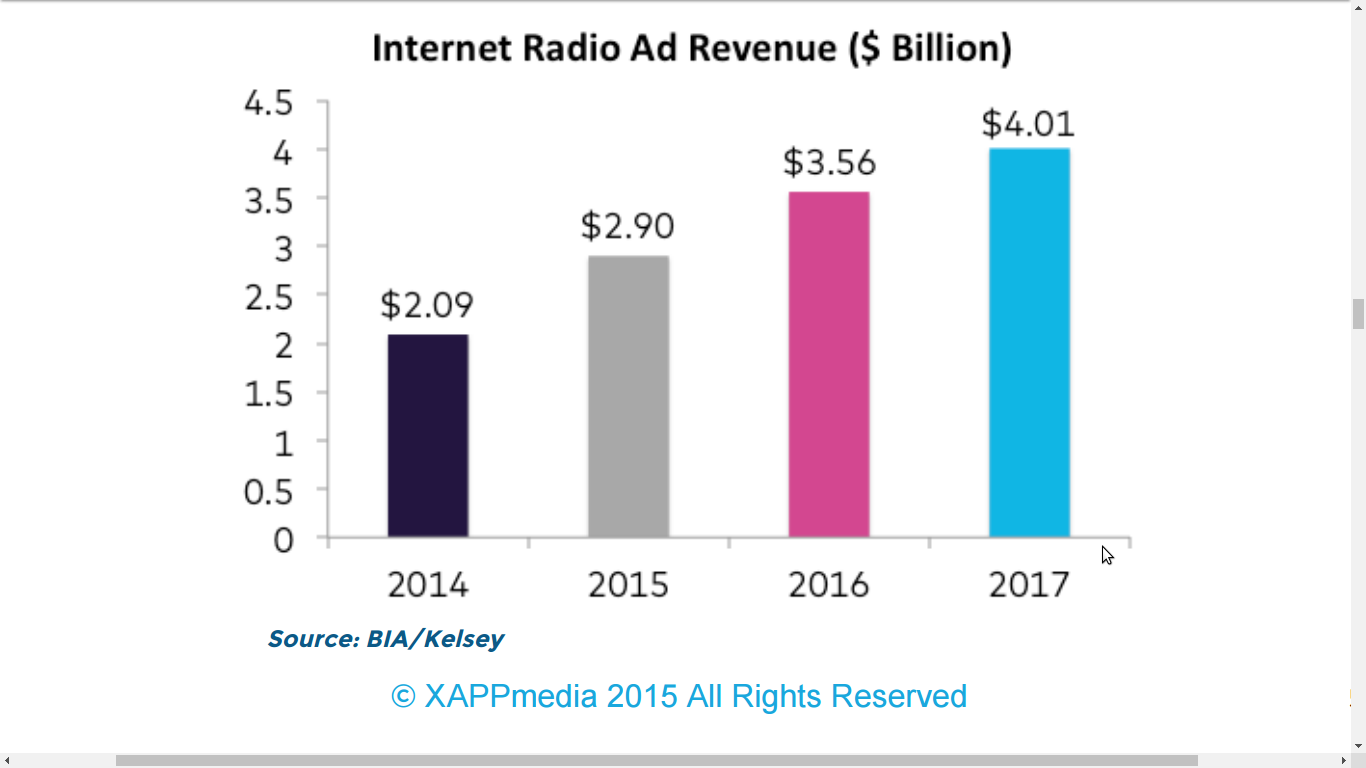
\includegraphics[width=\textwidth]{internet-radio-revenue}
 	\caption{Internet radio revenue from 2014 to 2017. Source \cite{edisonslide}}
 	\label{fig:InternetRadioRevenue}
\end{figure}
\begin{figure}[h]
	\centering
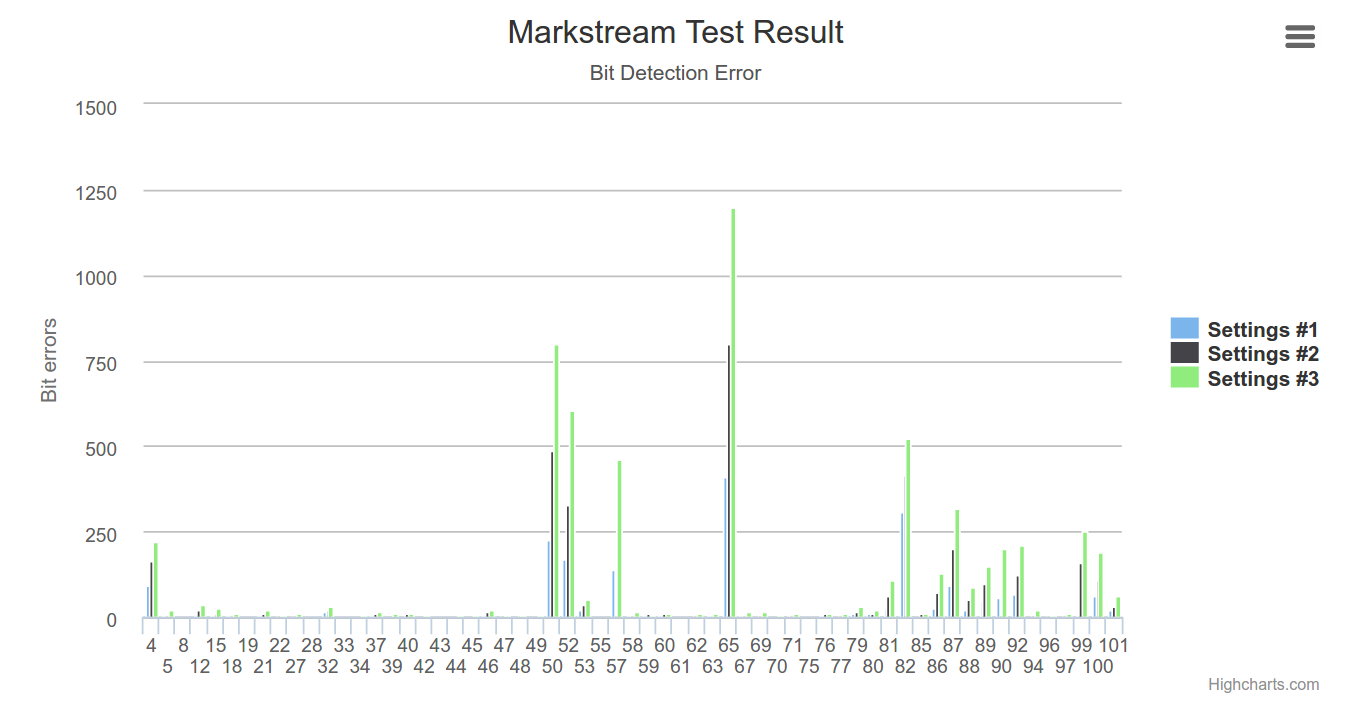
\includegraphics[width=\textwidth]{bdrmarkstream}
 	\caption{Bit detection rate test result.}
 	\label{fig:BDRMarkstream}
\end{figure}